%; whizzy chapter$B!!(B-dvi
% -initex iniptex -latex platex -format platex -bibtex jbibtex -fmt fmt
% $B0J>e(B whizzytex $B$r;HMQ$9$k>l9g$N@_Dj!#(B

%     Tokyo Debian Meeting resources
%     Copyright (C) 2012 Junichi Uekawa
%     Copyright (C) 2012 Nobuhiro Iwamatsu

%     This program is free software; you can redistribute it and/or modify
%     it under the terms of the GNU General Public License as published by
%     the Free Software Foundation; either version 2 of the License, or
%     (at your option) any later version.

%     This program is distributed in the hope that it will be useful,
%     but WITHOUT ANY WARRANTY; without even the implied warranty of
%     MERCHANTABILITY or FITNESS FOR A PARTICULAR PURPOSE.  See the
%     GNU General Public License for more details.

%     You should have received a copy of the GNU General Public License
%     along with this program; if not, write to the Free Software
%     Foundation, Inc., 51 Franklin St, Fifth Floor, Boston, MA  02110-1301 USA

%  preview (shell-command (concat "evince " (replace-regexp-in-string "tex$" "pdf"(buffer-file-name)) "&"))
% $B2hA|%U%!%$%k$r=hM}$9$k$?$a$K$O(Bebb$B$rMxMQ$7$F(Bboundingbox$B$r:n@.!#(B
%(shell-command "cd image201205; ebb *.png")

%%$B$3$3$+$i%X%C%@3+;O!#(B

\documentclass[mingoth,a4paper]{jsarticle}
\usepackage{monthlyreport}

% $BF|IU$rDj5A$9$k!"Kh7nJQ$o$j$^$9!#(B
\newcommand{\debmtgyear}{2012}
\newcommand{\debmtgmonth}{11}
\newcommand{\debmtgdate}{17}
% (+ (* (- 2012 2005) 12) 10 -1) started from zero
\newcommand{\debmtgnumber}{94}

\begin{document}

\begin{titlepage}
\thispagestyle{empty}
% $B%?%$%H%k%Z!<%8(B:$BJT=8I,MW$JItJ,$O:G=i$N%^%/%m$KHt$P$9$3$H(B

\vspace*{-2cm}
$BBh(B\debmtgnumber{}$B2s(B $BEl5~%(%j%"(B Debian $BJY6/2q;qNA(B\\
\hspace*{-2cm}

\includegraphics{image2012-natsu/dotdeb.pdf}\\
\hfill{}\debmtgyear{}$BG/(B\debmtgmonth{}$B7n(B\debmtgdate{}$BF|(B

% $B$3$3$O%"%C%W%G!<%H$9$k$3$H(B
% $BA43QJ8;z$K$7$J$$$H%U%)%s%H$N%5%$%:$,9g$o$J$$$N$GCm0U(B
% TODO(uekawa): $B$J$s$G$=$&$J$k$N$+3NG'(B
\rotatebox{10}{\fontsize{32}{32} {\gt $BFC=8(B: $B#D#e#b#c#o#n#f!!#R#e#p#o#r#t(B}}\\
\rotatebox{10}{\fontsize{32}{32} {\gt $BFC=8(B: $B7n4)#D#e#b#h#e#l#p#e#r(B}}\\

\vspace*{-2cm}
\hfill{}
\includegraphics[height=6cm]{image200502/openlogo-nd.eps}
\end{titlepage}

% Title should be in Japanese text so that we can use it as lint for PDF shiori.
\dancersection{$B$O$8$a$K(B}{$B>e@n(B $B=c0l(B}

\begin{multicols}{2}
 

 $B:#7n$N(BDebian$BJY6/2q$X$h$&$3$=!#$3$l$+$i(BDebian$B$N@$3&$K$"$7$rF'$_F~$l$k$H(B
 $B$$$&J}$b!"$9$G$K$I$C$W$j$H$D$+$C$F$$$k$H$$$&J}$b!"7n$K0l2s(BDebian$B$K$D$$(B
 $B$F8l$j$^$;$s$+!)(B

 Debian$BJY6/2q$NL\E*$O2<5-$G$9!#(B

 \begin{itemize}
 \item \underline{Debian Developer} ($B3+H/<T(B)$B$N0i@.!#(B
 \item $BF|K\8l$G$N!V(B\underline{$B3+H/$K4X$9$k>pJs(B}$B!W$r@0M}$7$F$^$H$a!"%"%C%W%G!<%H$9$k!#(B
 \item \underline{$B>l(B}$B$NDs6!!#(B
 \begin{itemize}
  \item $BIaCJ$P$i$P$i$J>l=j$K$$$k?M!9$,(B face-to-face $B$G=P2q$($k>l$rDs6!(B
	$B$9$k!#(B
  \item Debian $B$N$?$a$K$J$k$3$H$r8l$k>l$rDs6!$9$k!#(B
  \item Debian$B$K$D$$$F8l$k>l$rDs6!$9$k!#(B
 \end{itemize}
 \end{itemize}		

 Debian$B$NJY6/2q$H$$$&$3$H$G5f6KE*$K$O;22C<TA40w$,(BDebian Package$B$r$,$j$,$j(B
 $B$H:n$k%9!<%Q!<%O%C%+!<$K$J$C$?;Q$rLQA[$7$F$$$^$9!#>pJs$N6&M-!&3hMQ$rDL$7(B
 $B$F(B Debian$B$N:#8e$NG=F0E*$JE83+$X$NEZBf$H$7$F!"!V>l!W$H$7$F$N6u4V$rDs6!$9(B
 $B$k$N$,L\E*$G$9!#(B

\end{multicols}

\newpage

\begin{minipage}[b]{0.2\hsize}
 \definecolor{titleback}{gray}{0.9}
 \colorbox{titleback}{\rotatebox{90}{\fontsize{80}{80} {\gt $B%G%S%"%sJY6/2q(B} }}
\end{minipage}
\begin{minipage}[b]{0.8\hsize}
\hrule
\vspace{2mm}
\hrule
\begin{multicols}{2}
\tableofcontents
\end{multicols}
\vspace{2mm}
\hrule
\end{minipage}

\dancersection{$B;vA02]Bj(B}{$B>e@n(B $B=c0l(B}

$B:#2s$N;vA02]Bj$O0J2<$G$9(B:
\begin{enumerate}
 \item xxx
\end{enumerate}
$B$3$N2]Bj$KBP$7$FDs=P$$$?$@$$$?FbMF$O0J2<$G$9!#(B
\begin{multicols}{2}
{\small
%%; whizzy-master ../debianmeetingresume201208.tex
% $B0J>e$N@_Dj$r$7$F$$$k$?$a!"$3$N%U%!%$%k$G(B M-x whizzytex $B$9$k$H!"(Bwhizzytex$B$,MxMQ$G$-$^$9!#(B
%

\begin{prework}{ $BF|HfLn(B $B7<(B }

19$B<~G/$K$A$J$s$G!"$H$$$&$3$H$G$b$J$$$,!"(B
$B:#G/$O(B Haskell $B$N%i%$%V%i%j$r8x3+$9$kM=Dj$J$N$G!"(B
$B<+J,$G%Q%C%1!<%8%s%0$7$F%a%s%F%J$K$J$j$?$$!#(B
$B$"$H(B Debian Haskell $B%A!<%`$K$b;22C$7$F$$$-$?$$!#(B

\end{prework}

\begin{prework}{ $B$J$+$*$1$$$9$1(B }

$BJQ$o$i$:;H$$B3$1$^$9!#(B
$B$G!"$A$g$C$H$:$D!"(BContribute$B$7$F$$$3$&$H;W$C$F$^$9!#(B
\end{prework}

\begin{prework}{ $BLnEg!!5.1Q(B }

$BJzIi!'(B
$B!V2f$,$"$"(BDebian$B$N!ANO!J$j$g$/(B)$B$O$"$"$"$"@$3&$$$$$$%$%A%$%$%$%$%$%$(B
 $B%$!*!*!*!*!W$H$+8@$($k$HAGE($+$b(B...$B!J!A(B $B$NItJ,$OE,Ev$K(B...)
 
$B$A$g$C$H$0$i$$B>$N?M$,$d$C$?;v$,$J$$$3$H(B1$B$D$G$b(BDebian$B%M%?$G=PMh$?$i$$$$$J(B...$B!VL>>u$7$,$?$$2?$+$N%O!<%I%&%'%"!W$G(BDebian$BF0$+$7$F$_$k$H$+$+$J(B...

\end{prework}

\begin{prework}{ $B%-%?%O%i(B }

$B=tHL$NET9g$GGQ;_$5$l$F$7$^$C$?!"(B
$B2q<R$N(Bdebian$B%5!<%P$rI|3h$5$;$?$$$G$9$M!#(B

\end{prework}

\begin{prework}{ dictoss($B?yK\!!E5=<(B) }

kfreebsd$B$r;H$C$F3Z$7$_$J$,$i!"(Bdeb$B$7$F$$$-$^$9!#(B
\end{prework}

\begin{prework}{ $B@P0f0lIW(B }

DebConf$B$rF|K\$G3+:E$G$-$k$J$i$P!"@'Hs<B8=$5$;$?$$!#(B
\end{prework}

}
\end{multicols}

\dancersection{$B:G6a$N(BDebian$B4XO"$N%_!<%F%#%s%0Js9p(B}{$B>e@n(B $B=c0l(B}
\subsection{$BEl5~%(%j%"(BDebian$BJY6/2q(B93$B2sL\Js9p(B}

% (query-replace-regexp "<.*?>" "")
% (query-replace-regexp "^[	 ]\+" "")

%-------------------------------------------------------------------------------
\dancersection{}{}
%-------------------------------------------------------------------------------

%-------------------------------------------------------------------------------
\dancersection{Android $B7HBS$G(BBluetooth Tethering}{}
%-------------------------------------------------------------------------------

Android$B@_Dj2hLL!'(B
TODO

GNOME$B$N@_Dj2hLL(B
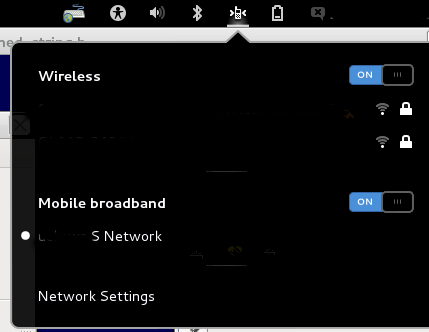
\includegraphics{image201211/bt1.png}

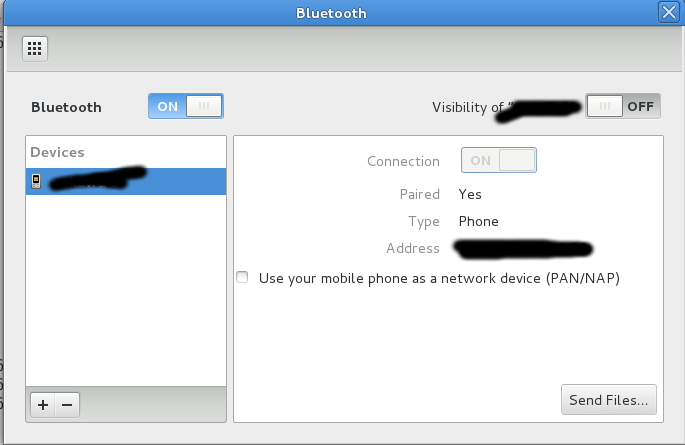
\includegraphics{image201211/bt2.png}

%-------------------------------------------------------------------------------
\dancersection{perf $B$G%Q%U%)!<%^%s%9%A%e!<%K%s%0(B}{}
%-------------------------------------------------------------------------------

\subsection{$B$O$8$a$K(B}

perf $B%3%^%s%I$O(B linux-base $B%Q%C%1!<%8$K$O$$$C$F$$$F$?$$$F$$$N4D6-$G$OI8=`(B
$B$G%$%s%9%H!<%k$5$l$F$$$k$N$G$9$,!"%+!<%M%k$K$"$C$?%P!<%8%g%s$N%P%$%J%j$r(B
$BDI2C$G%$%s%9%H!<%k$9$kI,MW$,$"$j$^$9!#(B

\begin{commandline}
 $ uname -r
3.2.0-3-amd64
 $ sudo apt-get install linux-tools-3.2
\end{commandline}

\subsection{perf stat}

$B$H$j$"$($:(B time $B%3%^%s%I$NBe$o$j$K$D$+$($=$&$J%D!<%k$H$7$F!"(B perf stat$B$,(B
$B$"$j$^$9!#(BCPU$B<~GH?t$,2DJQ$J%7%9%F%`$K$*$$$F%Q%U%)!<%^%s%9$NB,Dj$N$?$a$K<B(B
$B9T;~4V$N7WB,$H$$$&$N$OFq$7$$LdBj$J$N$G$9$,!"$3$l$G$_$k$H$@$$$?$$=EMW$J;X(B
$B?t$,8+$($F$-$^$9!#(B

\begin{commandline}
$ perf stat ./apt-index-cmd debian_dists_sid_main_binary-amd64_Packages  debian > /dev/null
 Performance counter stats for './apt-index-cmd debian_dists_sid_main_binary-amd64_Packages debian':

       1741.828818 task-clock                #    0.997 CPUs utilized          
               165 context-switches          #    0.000 M/sec                  
                 6 CPU-migrations            #    0.000 M/sec                  
            27,392 page-faults               #    0.016 M/sec                  
     4,990,934,326 cycles                    #    2.865 GHz                     [83.29%]
     1,681,297,382 stalled-cycles-frontend   #   33.69% frontend cycles idle    [83.27%]
     1,096,373,883 stalled-cycles-backend    #   21.97% backend  cycles idle    [66.62%]
     7,738,965,303 instructions              #    1.55  insns per cycle        
                                             #    0.22  stalled cycles per insn [83.51%]
     1,784,494,907 branches                  # 1024.495 M/sec                   [83.49%]
        32,701,183 branch-misses             #    1.83% of all branches         [83.32%]

       1.746581711 seconds time elapsed
\end{commandline}
  
\subsection{perf record}

\begin{commandline}
$ perf record ./apt-index-cmd debian_dists_sid_main_binary-amd64_Packages  debian > /dev/null
[ perf record: Woken up 1 times to write data ]
[ perf record: Captured and wrote 0.087 MB perf.data (~3800 samples) ]
$ ls -l perf.data
-rw------- 1 dancer dancer 93560 10$B7n(B 10 07:03 perf.data

\end{commandline}

perf record -g $B%*%W%7%g%s$r$D$1$k$H%3!<%k%0%i%U$b5-O?$9$k$h$&$G$9!#(B

\subsection{perf report}

$B%a%K%e!<7A<0$K$J$C$F$$$F!"5$$K$J$k%7%s%\%k$rA*Br$7$F%=!<%9%3!<%I$N%"%N%F!<(B
$B%7%g%s$r8+$k$3$H$,$G$-$^$9!#(B

\begin{commandline}
$ perf report
Events: 1K cycles                                                              
 18.65%  apt-index-cmd  apt-index-cmd        [.] available_parser::AptIndexSpiri
  7.38%  apt-index-cmd  libc-2.13.so         [.] _int_malloc
  6.64%  apt-index-cmd  libc-2.13.so         [.] malloc
  5.17%  apt-index-cmd  libstdc++.so.6.0.17  [.] std::string::_M_replace_aux(uns
  4.03%  apt-index-cmd  libc-2.13.so         [.] _int_free
  4.02%  apt-index-cmd  libstdc++.so.6.0.17  [.] __cxxabiv1::__vmi_class_type_in
  3.81%  apt-index-cmd  libstdc++.so.6.0.17  [.] std::string::_M_mutate(unsigned
  3.59%  apt-index-cmd  libstdc++.so.6.0.17  [.] std::ctype<char> const& std::us
  3.00%  apt-index-cmd  libc-2.13.so         [.] __strcmp_sse42
  2.74%  apt-index-cmd  apt-index-cmd        [.] boost::detail::function::functi
  2.72%  apt-index-cmd  libstdc++.so.6.0.17  [.] __dynamic_cast
  2.67%  apt-index-cmd  libc-2.13.so         [.] free
  2.46%  apt-index-cmd  libc-2.13.so         [.] __memcmp_sse4_1

[$B%(%s%?!<$r2!$9(B]

available_parser::AptIndexSpirited::MakeIndex()::{lambda(std::vector<char, std::
    0.00 :          40368a:       je     4036ac <available_parser::AptIndexSpir
         :                                                                     
         :          const std::string& get() const { return my_string_; }      
         :                                                                     
         :          // for 'map' comparison.                                   
         :          bool operator<(const OrderedHashedString& b) const {       
         :            if (ordered_hash_ == b.ordered_hash_) {                  
    2.87 :          40368c:       mov    0x28(%rbx),%rdx                       
         :              return my_string_ < b.my_string_;                      
         :            } else {                                                 
         :              return ordered_hash_ < b.ordered_hash_;                
   34.96 :          403690:       cmp    %rbp,%rdx                             
    1.43 :          403693:       setb   %cl                                   
         :                                                                     
         :          const std::string& get() const { return my_string_; }      
         :                                                                     
         :          // for 'map' comparison.                                   
         :          bool operator<(const OrderedHashedString& b) const {       
         :            if (ordered_hash_ == b.ordered_hash_) {                  
  
 \end{commandline}

\printindex

\cleartooddpage

\vspace*{15cm}
\hrule
\vspace{2mm}

\includegraphics[width=2cm]{image200502/openlogo-nd.eps}
\noindent \Large \bf Debian $BJY6/2q;qNA(B\\
\noindent \normalfont \debmtgyear{}$BG/(B\debmtgmonth{}$B7n(B\debmtgdate{}$BF|(B \hspace{5mm}  $B=iHGBh(B1$B:~H/9T(B\\
\noindent \normalfont $BEl5~%(%j%"(B Debian $BJY6/2q(B $B!JJT=8!&0u:~!&H/9T!K(B\\
\hrule

\end{document}
